\documentclass{beamer}
\usepackage{ulem}
\usepackage{tikz}
\usepackage{booktabs}
 \usepackage{graphicx,threeparttable,caption}
\usetikzlibrary{shapes,snakes}
\usepackage[beamer,customcolors]{hf-tikz}
\usepackage{nicematrix}
\usepackage{xcolor}
\usepackage{makecell}
\usepackage{array}
\usepackage{csquotes}
\usepackage{csquotes}
\usepackage{minted}
\captionsetup{labelformat=empty,labelsep=none}

\graphicspath{ {./png/} }

\usetikzlibrary{
    arrows,
    arrows.meta,
    shapes,
    positioning,
    shadows,
    trees,
    calc
}

\tikzset{%
    >={Latex[width=2mm,length=2mm]},
    % Specifications for style of nodes:
    plain/.style = {},
    base/.style = {
        plain,
        rectangle, rounded corners, draw=black,
        minimum width=1cm, minimum height=1cm,
        text centered, font=\sffamily\tiny\bfseries,
        fill=white, align=center
    },
    app/.style = {base, ellipse},
    data/.style = {base, fill=gray!30},
    action/.style = {base, circle, fill=red!30},
    note/.style = {app, fill=yellow},
    hl/.style={
    set fill color=red!80!black!40,
    set border color=red!80!black
    }
}


\AtBeginSection[]{
  \begin{frame}
  \vfill
  \centering
  \begin{beamercolorbox}[sep=8pt,center,shadow=true,rounded=true]{title}
    \usebeamerfont{title}\insertsectionhead\par%
  \end{beamercolorbox}
  \vfill
  \end{frame}
}
%\usecolortheme[orchid]{structure}
\usetheme[hideothersubsections]{PaloAlto}
\makeatletter
\patchcmd{\csq@bquote@i}{{#6}}{{\emph{#6}}}{}{}
\makeatother
%\usecolortheme{orchid}
%\usefonttheme{professionalfonts}
\newcommand{\soutthick}[1]{%
   \textcolor{red}{
   \renewcommand{\ULthickness}{1pt}%
      \sout{#1}%
   \renewcommand{\ULthickness}{.4pt}% Resetting to ulem default
   }
}
\newcommand{\centered}[1]{\begin{tabular}{l} #1 \end{tabular}}
\setbeamertemplate{section in toc}[square]
\setbeamertemplate{subsection in toc}[square]
\setbeamertemplate{secion in sidebar}[shaded]
\setbeamertemplate{items}[square]
\setbeamercovered{transparent} 

\title[]{Introduction to Computational Social Science}
\subtitle{Introduction to Data Science}
\author[]{Mikołaj Biesaga\\ \small{\color{blue}{\href{mailto:m.biesaga@uw.edu.pl}{m.biesaga@uw.edu.pl}}}}
\institute{
\includegraphics[width = 4 cm]{uw.png}}
\date{\today}
\begin{document}
\begin{frame}
   \titlepage
\end{frame}
\section[Rules of Engagement]{Rules of Engagement}

\begin{frame}
    \frametitle{Workflow}
    \begin{enumerate}
        \only<1>{
        \item Presentation of the basic concepts in the classroom
        \item Exercises in the classroom
        \item Homework assignments requiring modifying the work done in the classroom
        \item Final research project
        }
        \only<2>{
        \item \soutthick{Presentation of the basic concepts in the classroom}
        \item \soutthick{Exercises in the classroom}
        \item \soutthick{Homework assignments requiring modifying the work done in the classroom}
        \item \soutthick{Final research project}
        }
        \only<3>{
        \item Presentation of the key concepts in the classroom
        \item Presentation of the selected papers using computational methods
        \item Students presentations of papers using computational methods
        }
        \end{enumerate}
\end{frame}
\begin{frame}
    \frametitle{Assessment Criteria}
    \only<1,2>{
        \begin{itemize}
            \item The final grade will be determined based on \alert<1>{6 homework
            assignments} and \alert<1>{written project proposal}.
            \item The first 4 homework (after classes: 2, 3, 4, and 5) will be scored from 0 to 10 points and the
            other two (after classes: 12 and 15) from 0 to 15 points.
            \item The research project will require writing a research proposal that uses the tools and methods discussed during the class. It will be scored from 0 to 85 points.
            \item Grading criteria:
        \begin{description}
            \item [5\phantom{+} --] => 140 points
            \item [4+ --] 132 - 139 points
            \item [4\phantom{+} --] 117 - 131 points
            \item [3+ --] 109 - 116 points
            \item [3\phantom{+} --] 93 - 108 points
            \item [2\phantom{+} --] =< 92 points
        \end{description}
        \end{itemize}
    }
    \only<2>{
        \begin{tikzpicture}[overlay]
        \draw [color = red, thick] (0,0) -- (10.2,7.8);
        \draw [color = red, thick](0,7.8) -- (10.2,0);
        \end{tikzpicture}
    }
    \only<3>{
        \begin{block}{}
            The final grade will be determined based on \alert{the prepared
            presentation} and \alert{questions asked during others presentations}.
        \end{block}
    }
\end{frame}
\begin{frame}
    \frametitle{Office Hours, Emails, Presentations, etc.}
    \begin{description}[Google Classroom:]
        \item [Office Hours:] write me an email before coming
        \item [Emails:] the official info will go through emails
        \item [GitHub:] \soutthick{scripts (notebooks) will be posted on GitHub}
        \item [Google Classroom:] materials and presentations will be posted on
        Google Classroom
    \end{description}
    \alert{I will try to answer your inquiries as soon as possible but do not
    count on an immediate response, especially right before the deadlines.}
\end{frame}


\section[CSS]{Computational Social Science}

\begin{frame}
    \frametitle{What is Computational Social Science?}
    \begin{definition}{}
        In the most general sense \emph{Computational Social Science} is a data-driven approach that uses computational methods in studying social phenomena.
    \end{definition}
    \begin{definition}{}
        \emph{Data Science} on the other hand is a broader term than Computational Social Science. It describes the theory and practice of extracting knowledge and insight from data.
    \end{definition}
\end{frame}

\begin{frame}{General interest in data science}
    \begin{figure}
    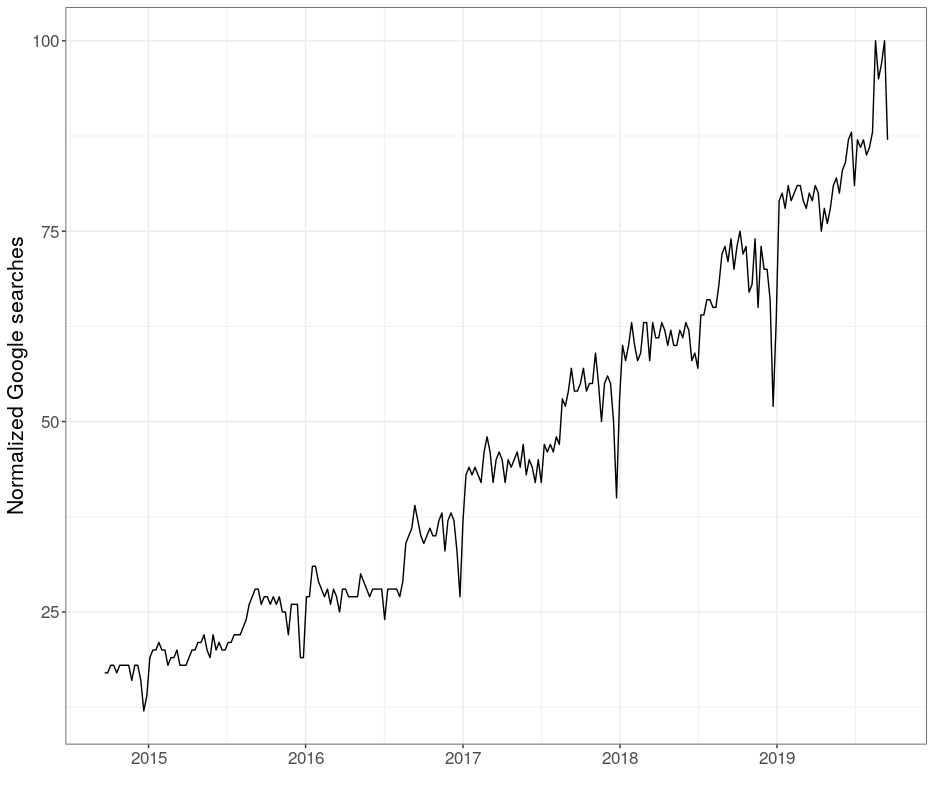
\includegraphics[width = .8\framewidth]{png/ds-searches.png}
    \caption{Growth of "data science" Google search}
    \end{figure}
\end{frame}

\subsection{Research Methods}

\begin{frame}
    \frametitle{Traditional Research Methods}
        \only<+>{
            \begin{itemize}
                \item surveys
                \item observational studies
                \item experiments
                \item case studies
                \item event sampling methodology (diaries)
                \item interviews
                \item focus groups
                \item meta-analysis
                \item desk research
            \end{itemize}}
        \only<+>{
            \resizebox{\textwidth}{!}{
                \begin{tabular}{l | c | c | c | c | c | c }
                Id & Sex & Age & Condition & Variable A & Variable B & Variable C\\
                \hline \hline
                AAA & M & 24 & exp & 55:53 & 3 & apple\\
                AAB & F & 22 & exp & 53:47 & 2 & banana\\
                AAC & F & 28 & con & n/a   & 4 & banana\\
                AAD & M & 21 & con & 54:35 & 3 & banana
                \end{tabular}}
        }
\end{frame}

\begin{frame}
    \frametitle{Computational methods}
    \setbeamercovered{transparent}
    \begin{itemize}
        \item<1> extraction of unstructured data from external digital (i.e. web-based) sources
        \begin{itemize}
            \item<1> webscraping (extraction of data from existing webpages)
            \item<1> extracting data from web APIs (i.e. Twitter)
        \end{itemize}
        \item<1> analysis of textual data (natural language processing - NLP)
        \item<1> network and relational data analysis
        \item<1> working with big datasets (that do not fit into the RAM of a single computer), in-database computations, distributed computing, etc.
        \item<1> computer simulations
        \item<1> online experiments (experiments based on online games etc.)
    \end{itemize}
\end{frame}

\section[Data]{Data}

\subsection[Data Sources]{Data Sources}
\begin{frame}
    \setbeamercovered{transparent}
    \frametitle{Data Sources}
    \only<+>{
        \begin{figure}
            
\includegraphics[scale=.35]{png/data_everywhere.png}
        \end{figure}}
    \only<+>{
        \begin{figure}
            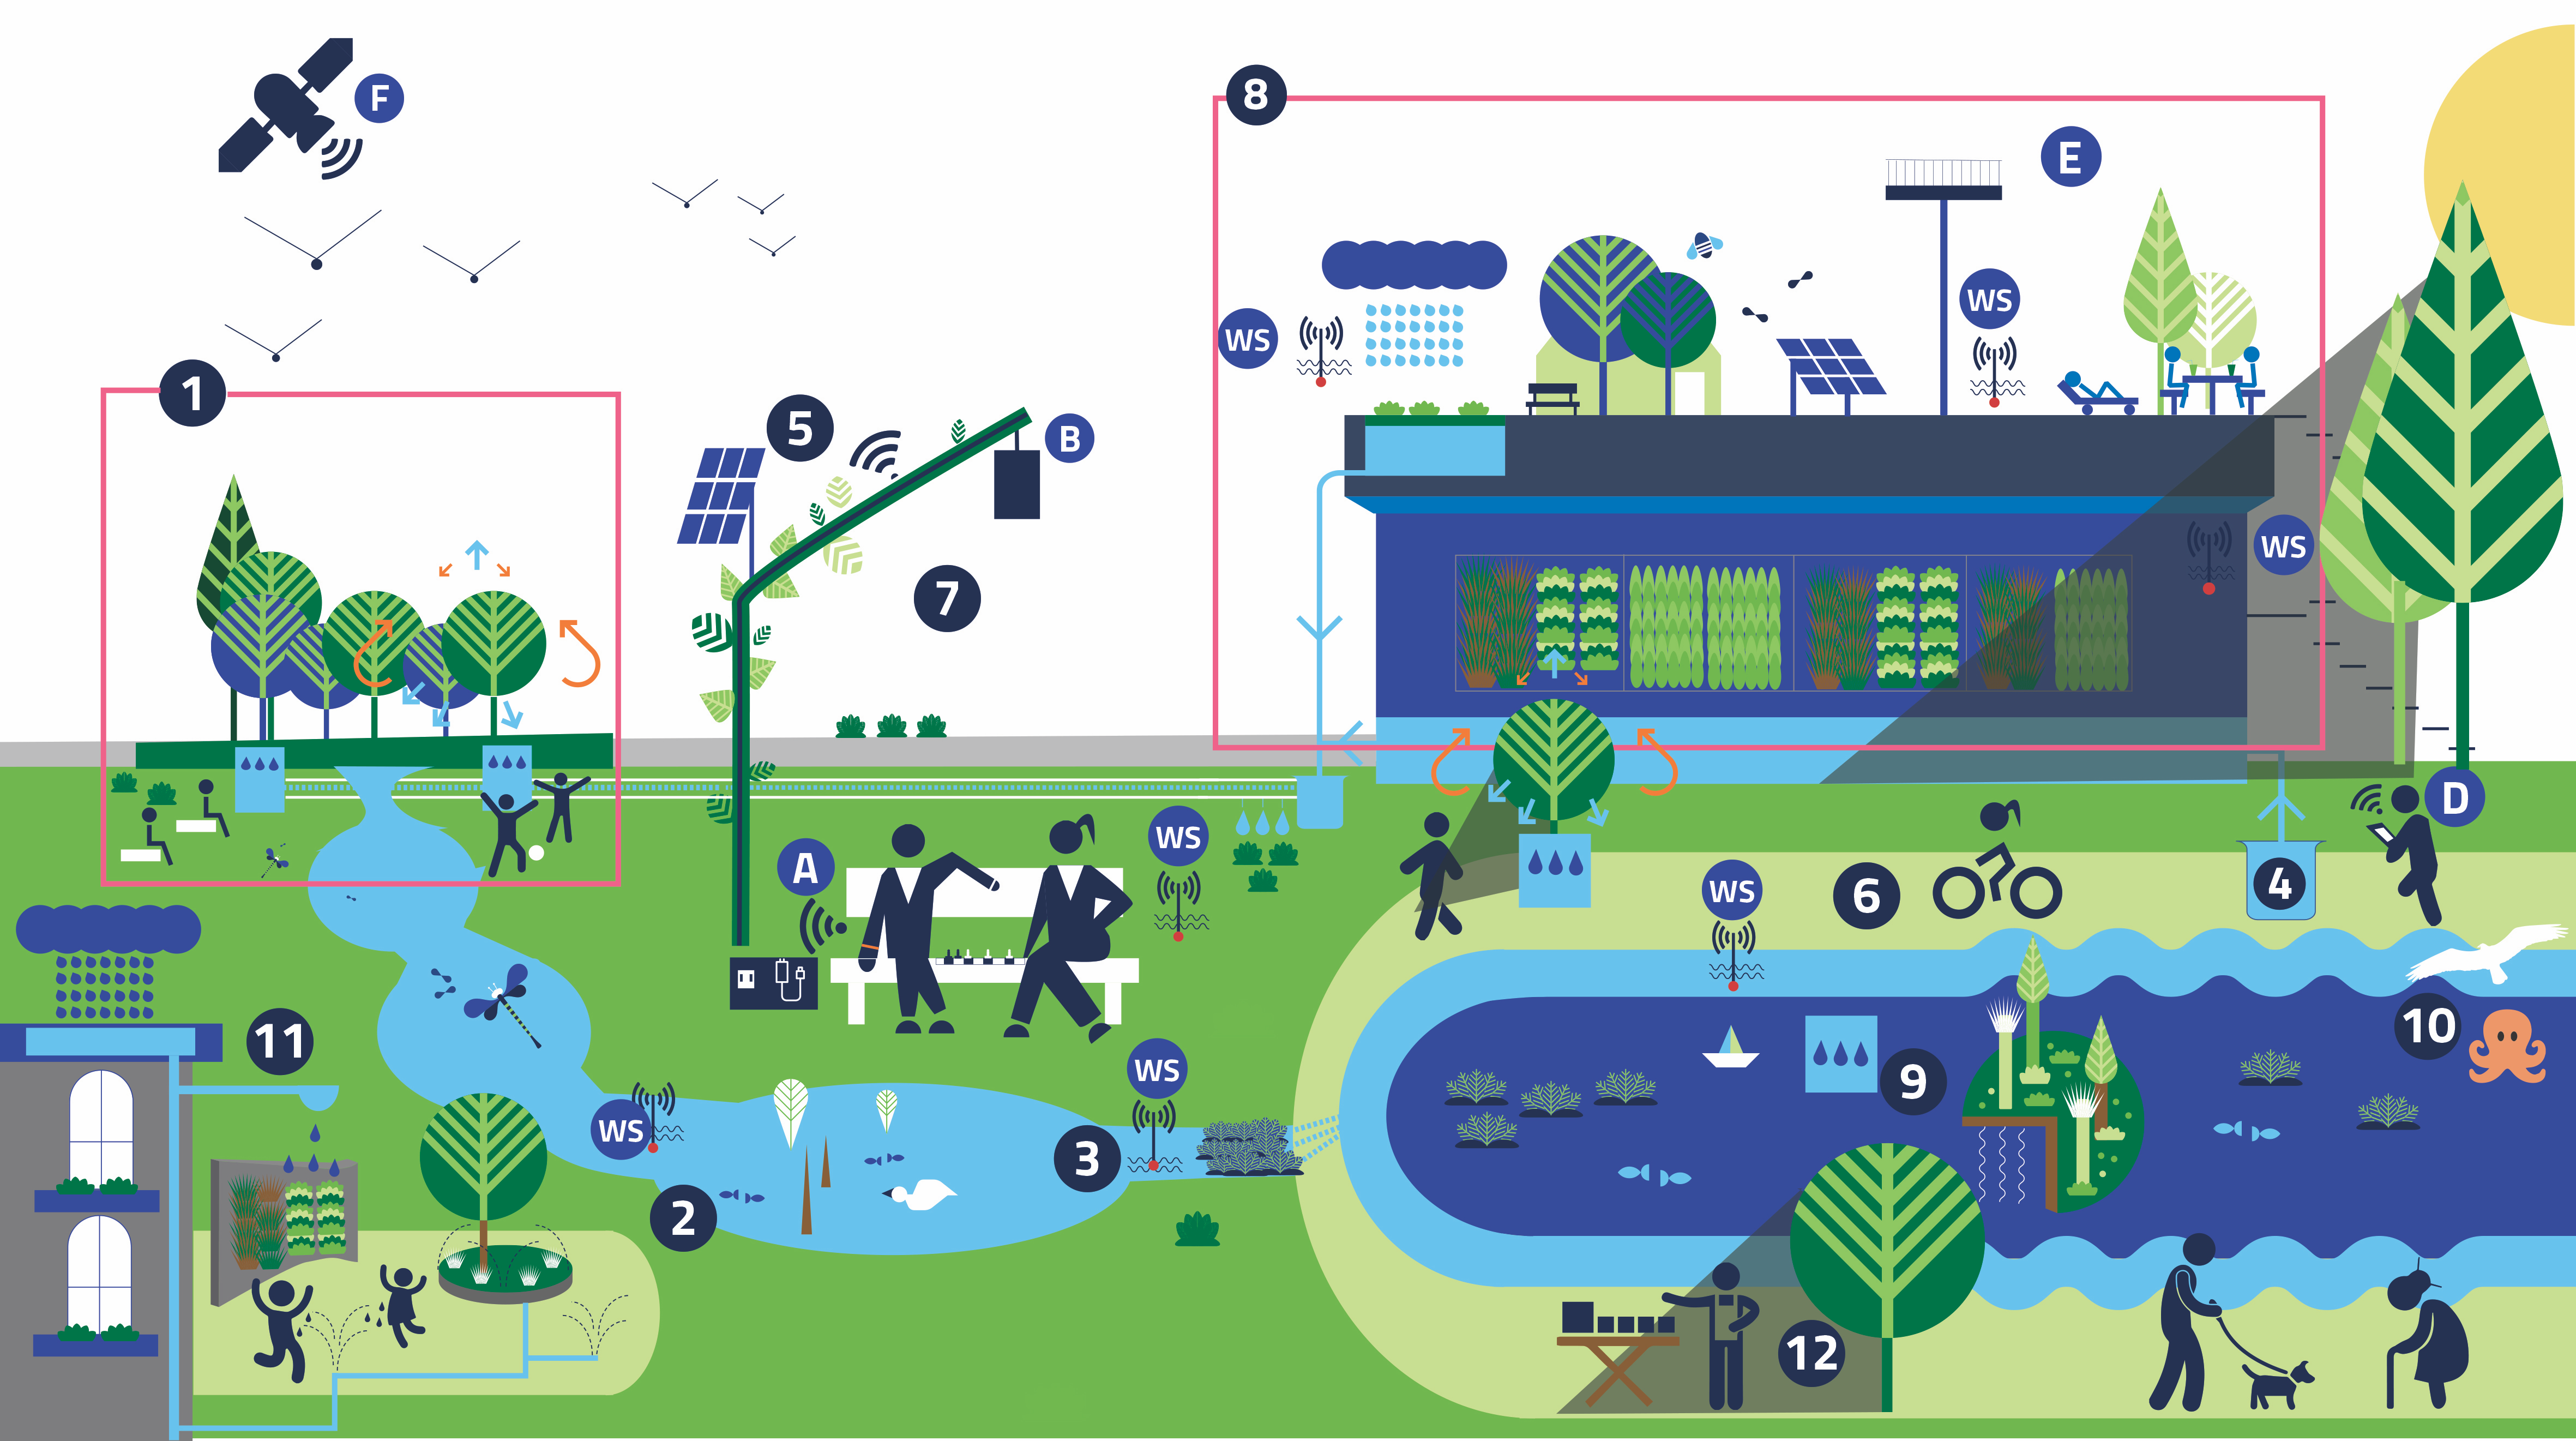
\includegraphics[width = \textwidth]{png/mierzenie.png}
        \end{figure}
    }
    \only<+>{
        \begin{figure}
            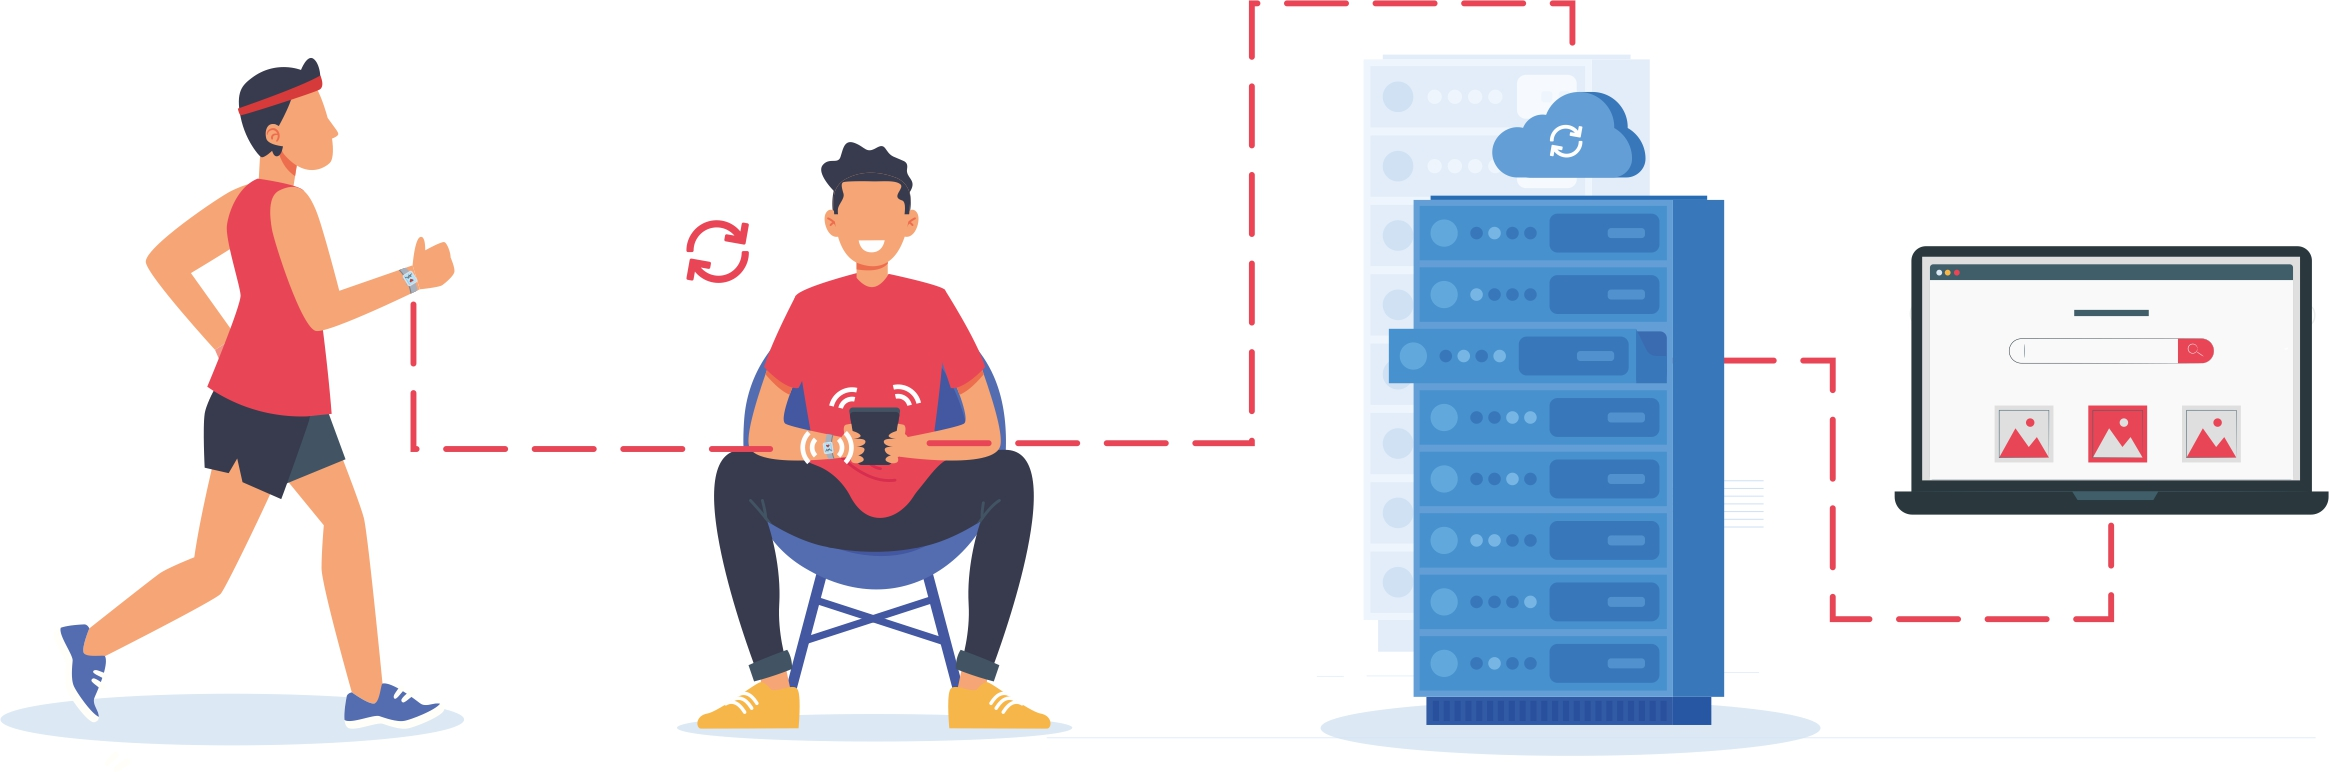
\includegraphics[scale = .5]{png/tracker.jpg}
        \end{figure}
    }
    \only<+>{
        \begin{itemize}
            \item<4> webpages
            \item<4> social media
            \item<4> smart devices
            \item<4> digital behavioral data
            \item<4> mobile phone networks
            \item<4> goverment data
            \item <4>...
        \end{itemize}
        \action<4>{\alert{The fact that you can get the data does not mean you should.}}
    }
\end{frame}

\subsection{Webscraping}

\begin{frame}
    \frametitle{Webscraping}
    \only<+>{
        \begin{figure}
            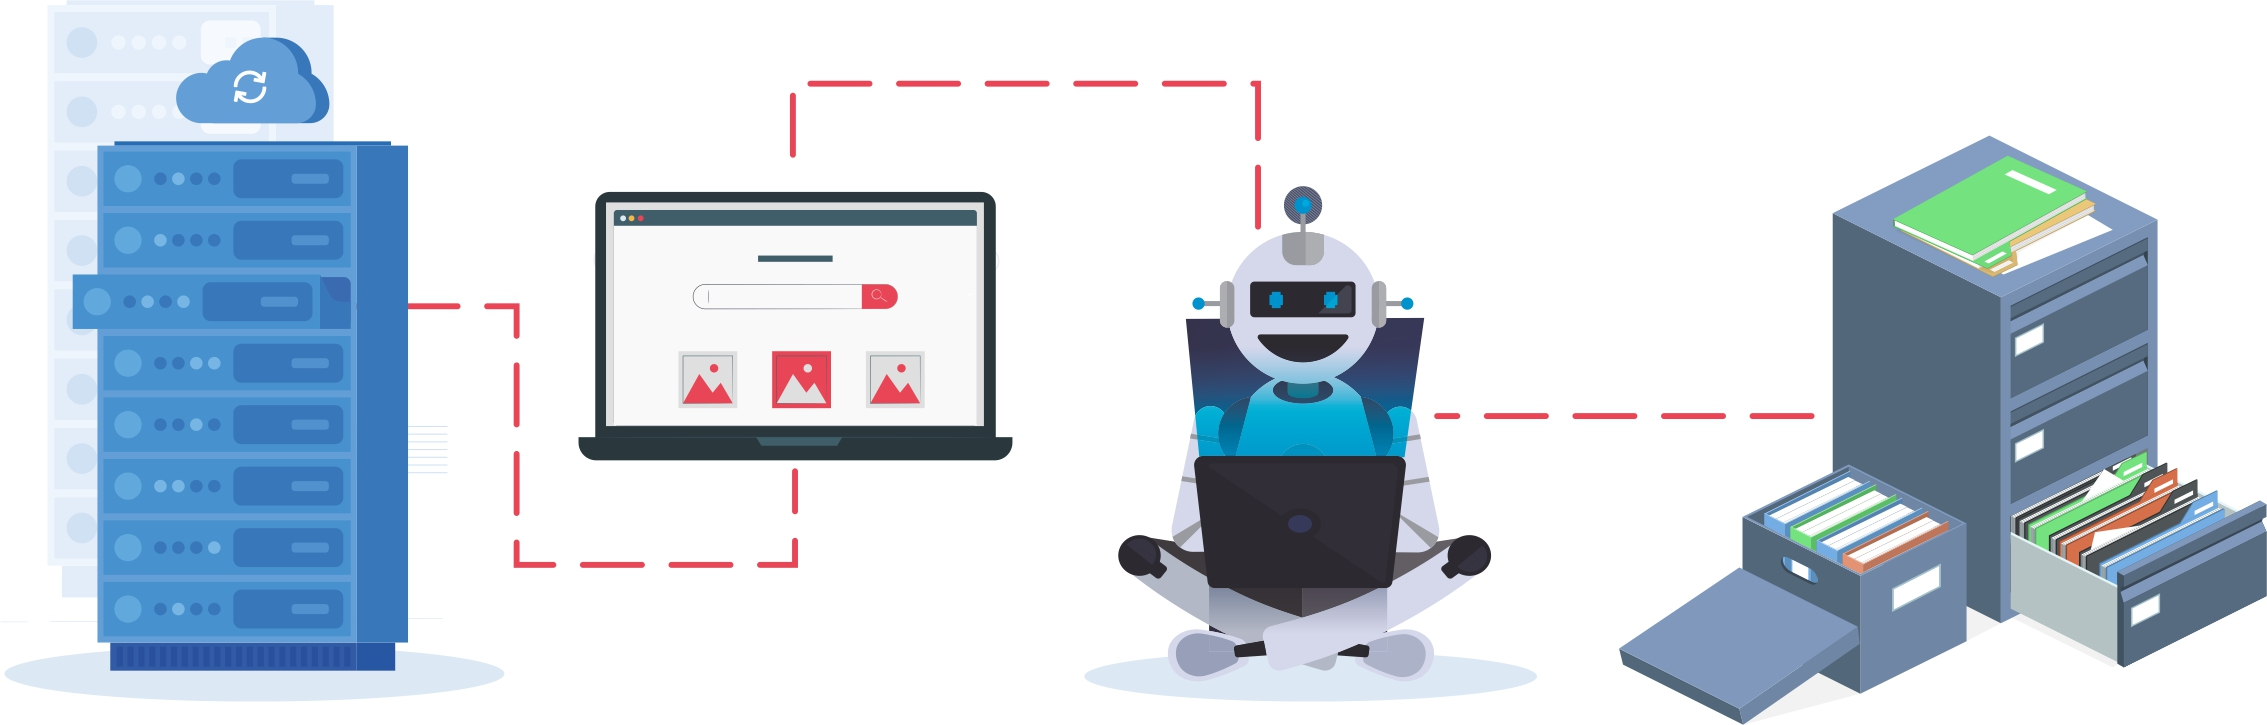
\includegraphics[scale = .5]{png/webscraping.jpg}
        \end{figure}
    }
    \only<+>{
        \begin{figure}
            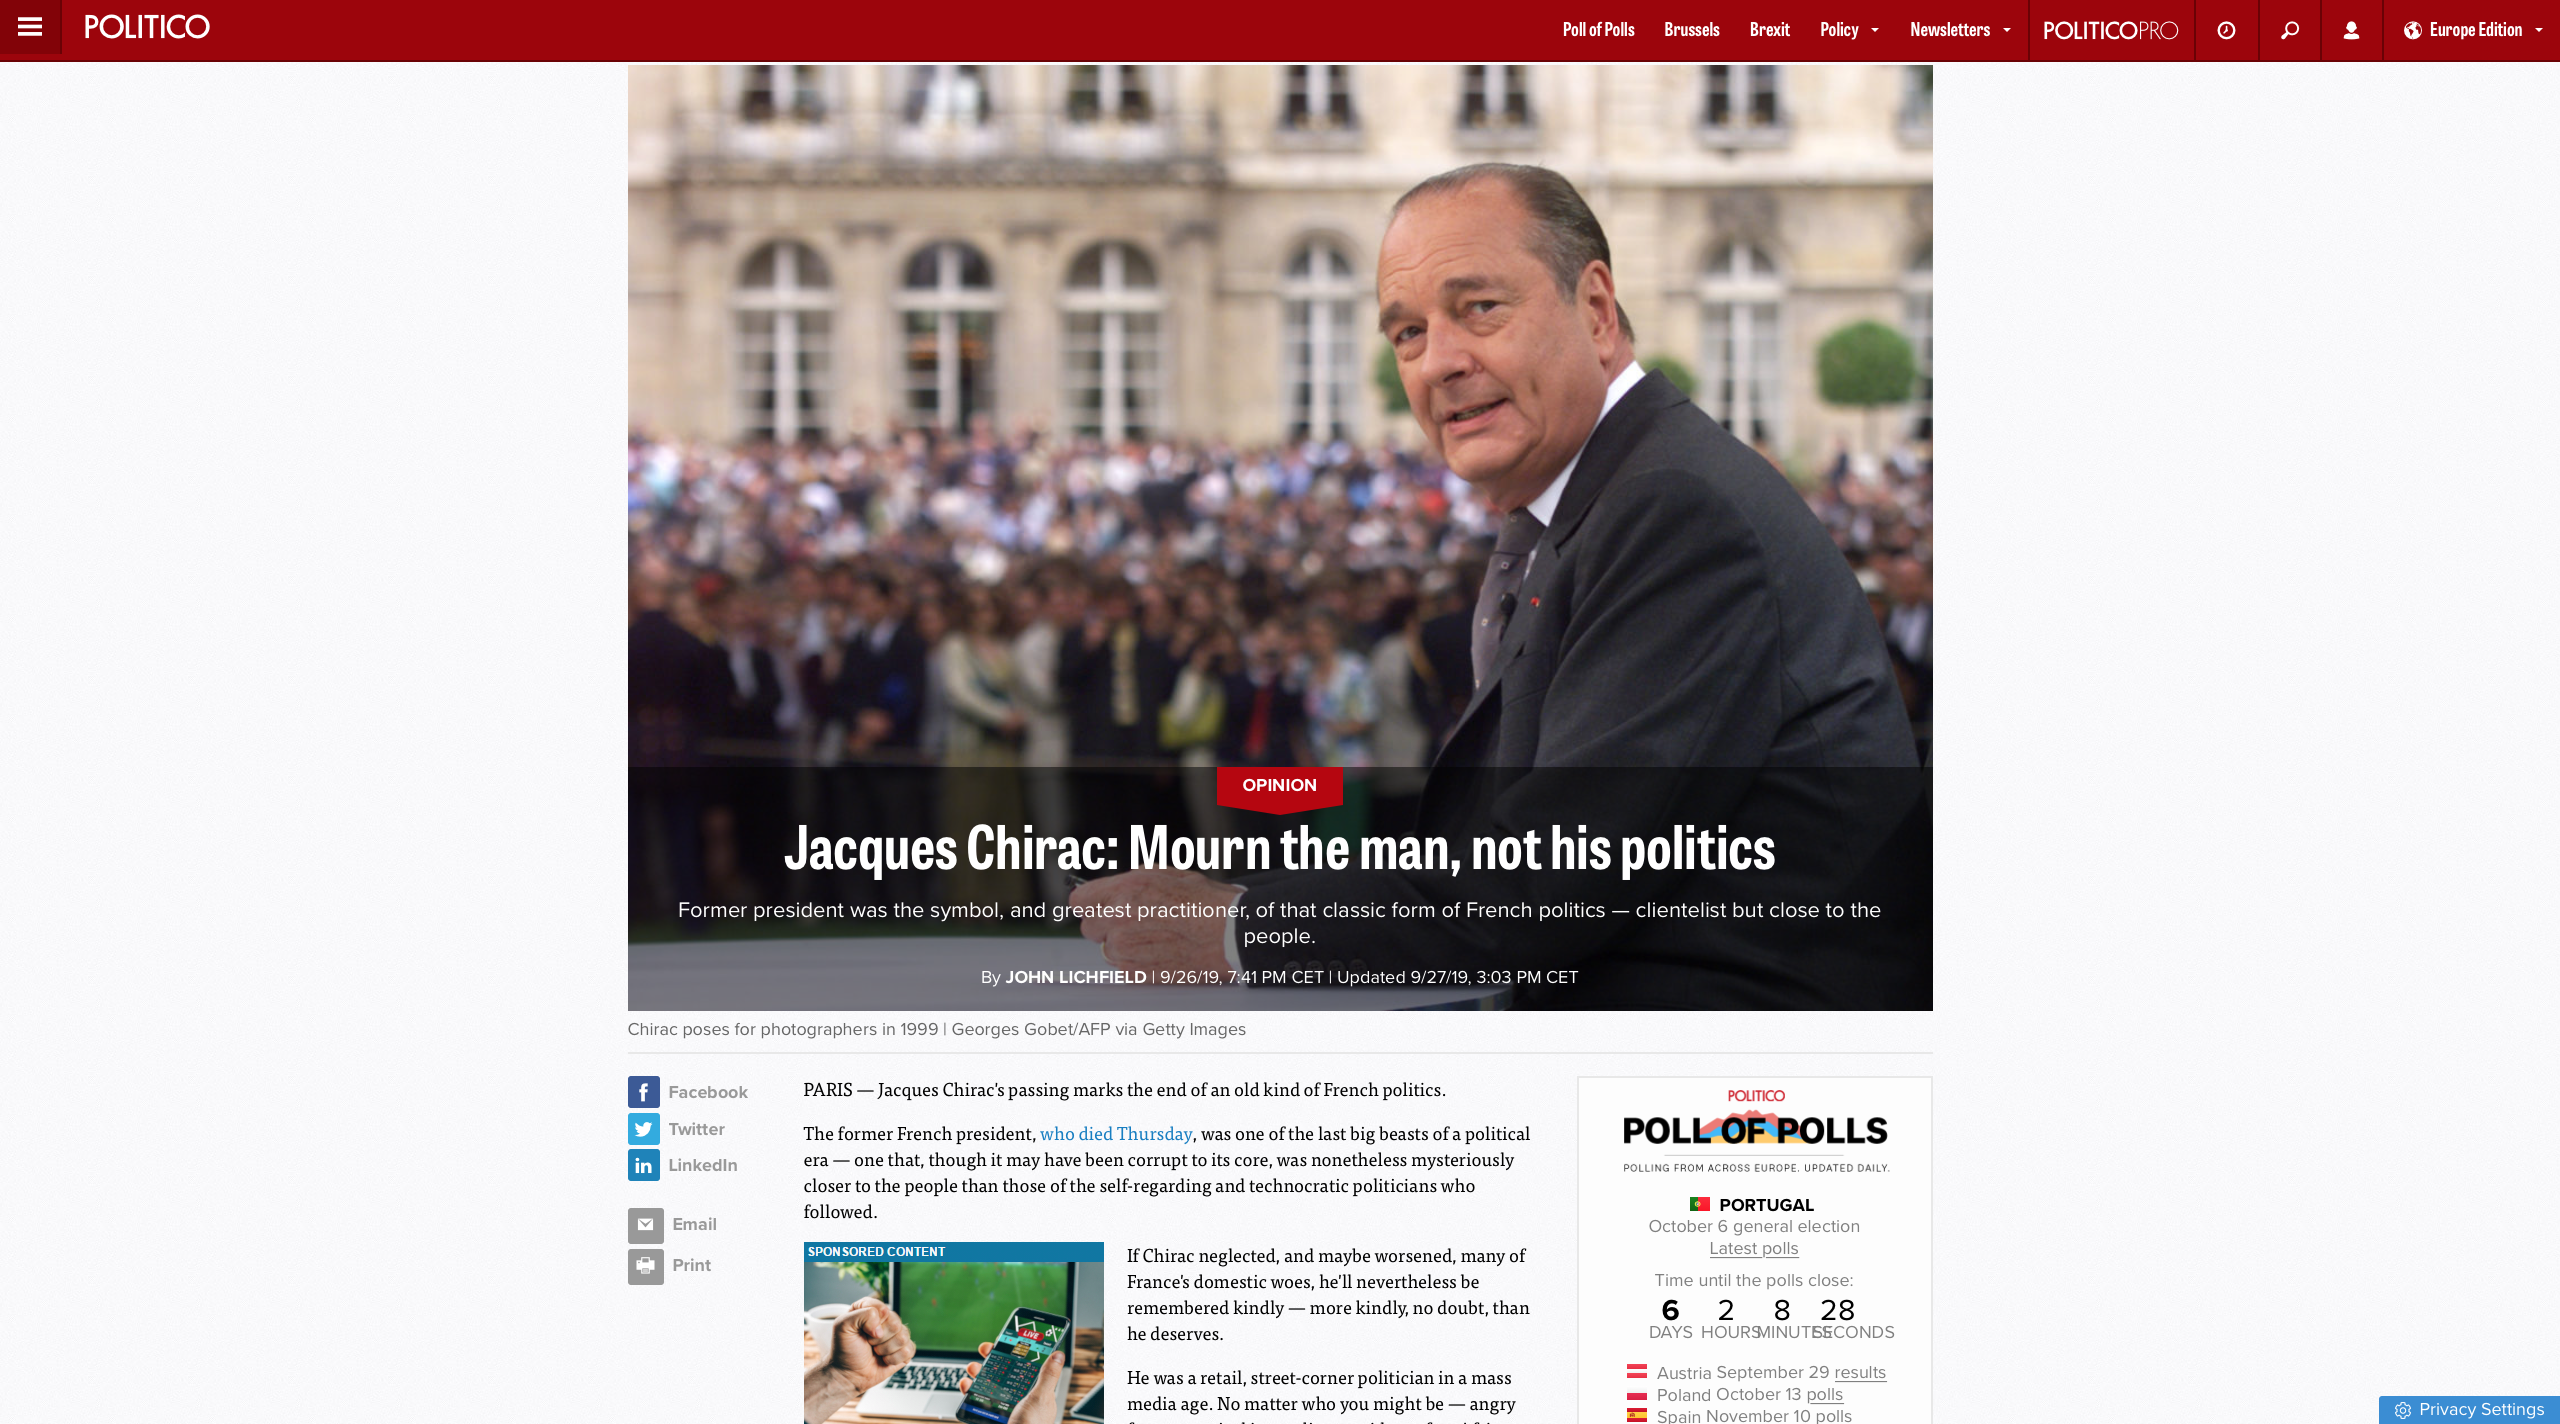
\includegraphics[scale = .22]{png/politico.png}
            \caption{from \textcolor{blue}{\href{https://www.politico.eu/article/jacques-chirac-mourn-the-man-not-his-politics/}{POLITICO Europe}}}
        \end{figure}
    }
    \only<+>{
        \begin{definition}
            \emph{Webscraping} is a process of (usually) automatic extraction of data from a website or multiple websites. In other words, it is a form of copying the data from a website into a local database or spreadsheet.
        \end{definition}
    }
\end{frame}

\subsection{HTML}

\begin{frame}
    \frametitle{HyperText Markup Language}
    \begin{definition}{}
        \emph{HyperText Markup Language} (HTML) is the standard markup language for
        documents designed to be displayed in a web browser. It defines the
        content and structure of web content. It is often assisted by
        technologies such as Cascading Style Sheets (CSS) and scripting
        languages such as JavaScript.
    \end{definition}
\end{frame}

\begin{frame}[fragile]
\frametitle{HyperText Markup Language}
\begin{minted}[fontsize=\footnotesize]{html}
<!DOCTYPE html>
<html>
    <head>
        <title>
            Justyna Kowalczyk fandom
        </title>
    </head>
    <body>
        <h1>
            Why Justyna Kowalczyk is the best?
        </h1>
        <p>
            Because she is just <b>the best</b> cross-country 
            skier in the history of the sport. You can learn
            more about her amazing achievements visiting
            her Wikipedia webpage:
            https://pl.wikipedia.org/wiki/Justyna_Kowalczyk.
        </p>
    </body>
</html>
\end{minted}
\end{frame}

\begin{frame}
    \frametitle{HyperText Markup Language}
    \only<+>{
        \framesubtitle{What are tags?}
        Tags are used to mark up the start of an HTML element and they are enclosed
        in \textbf{angle brackets}. The most important is the <html> tag. Inside
        this tag, between <html> and </html> all other elements live. In the 
        example from the previous slide we had the following tags:
        \begin{itemize}
            \item {<head></head>} -- element contains meta-information about the document
            \item {<title></title>} -- element specifies a title for the document
            \item {<body></body>} -- element contains the visible page content
            \item {<h1></h1>} -- element defines a large heading
            \item {<p></p>} -- element define a paragraph
            \item {<b></b>} -- element define a boldface
        \end{itemize}
    }
    \only<+>{
        \centering
        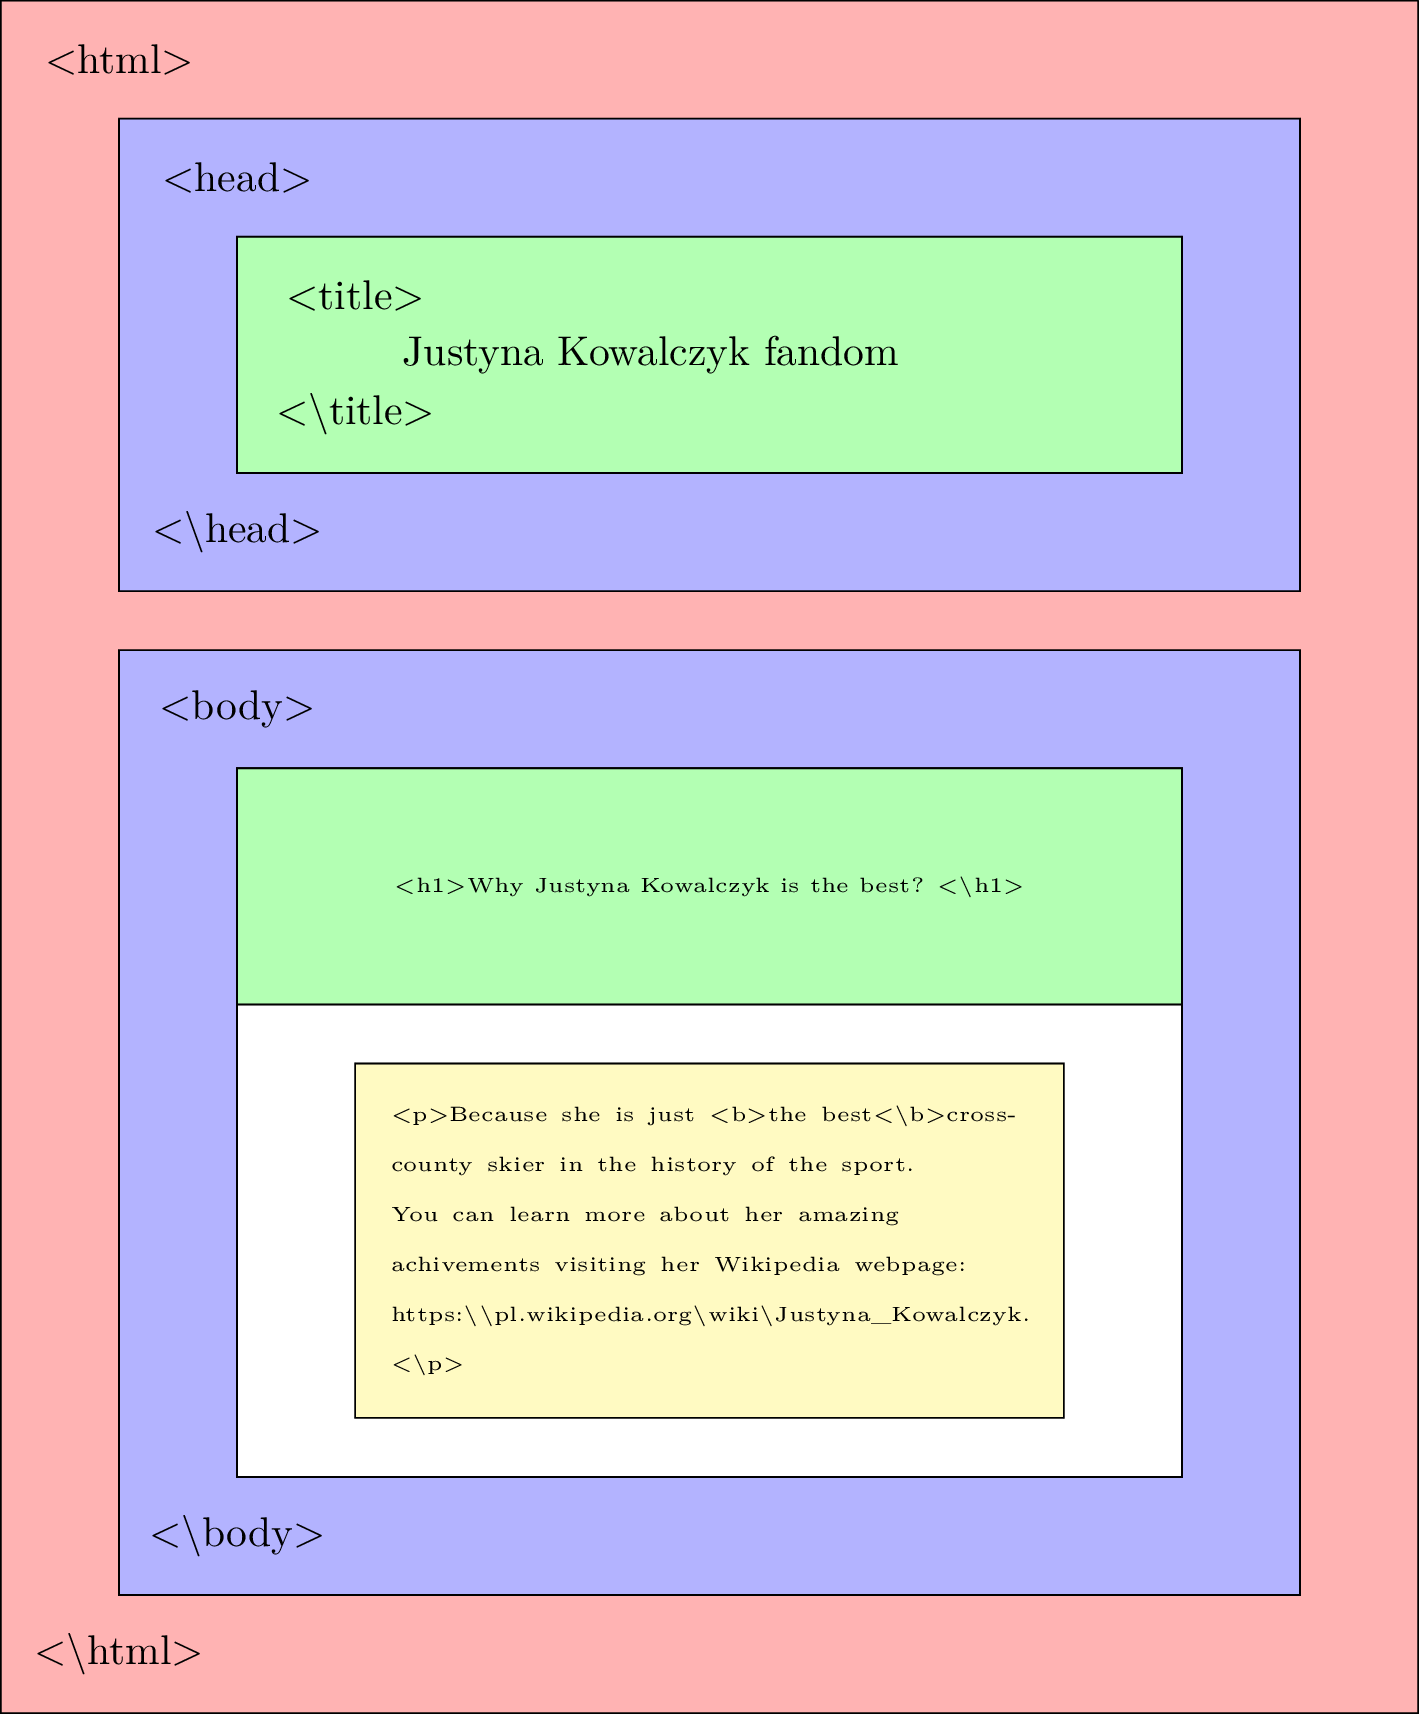
\includegraphics[width = .6\textwidth]{dom.png}
    }
\end{frame}

\subsection{API}

\begin{frame}
    \frametitle{Application Programming Interface}
    \only<+>{
        \begin{figure}
            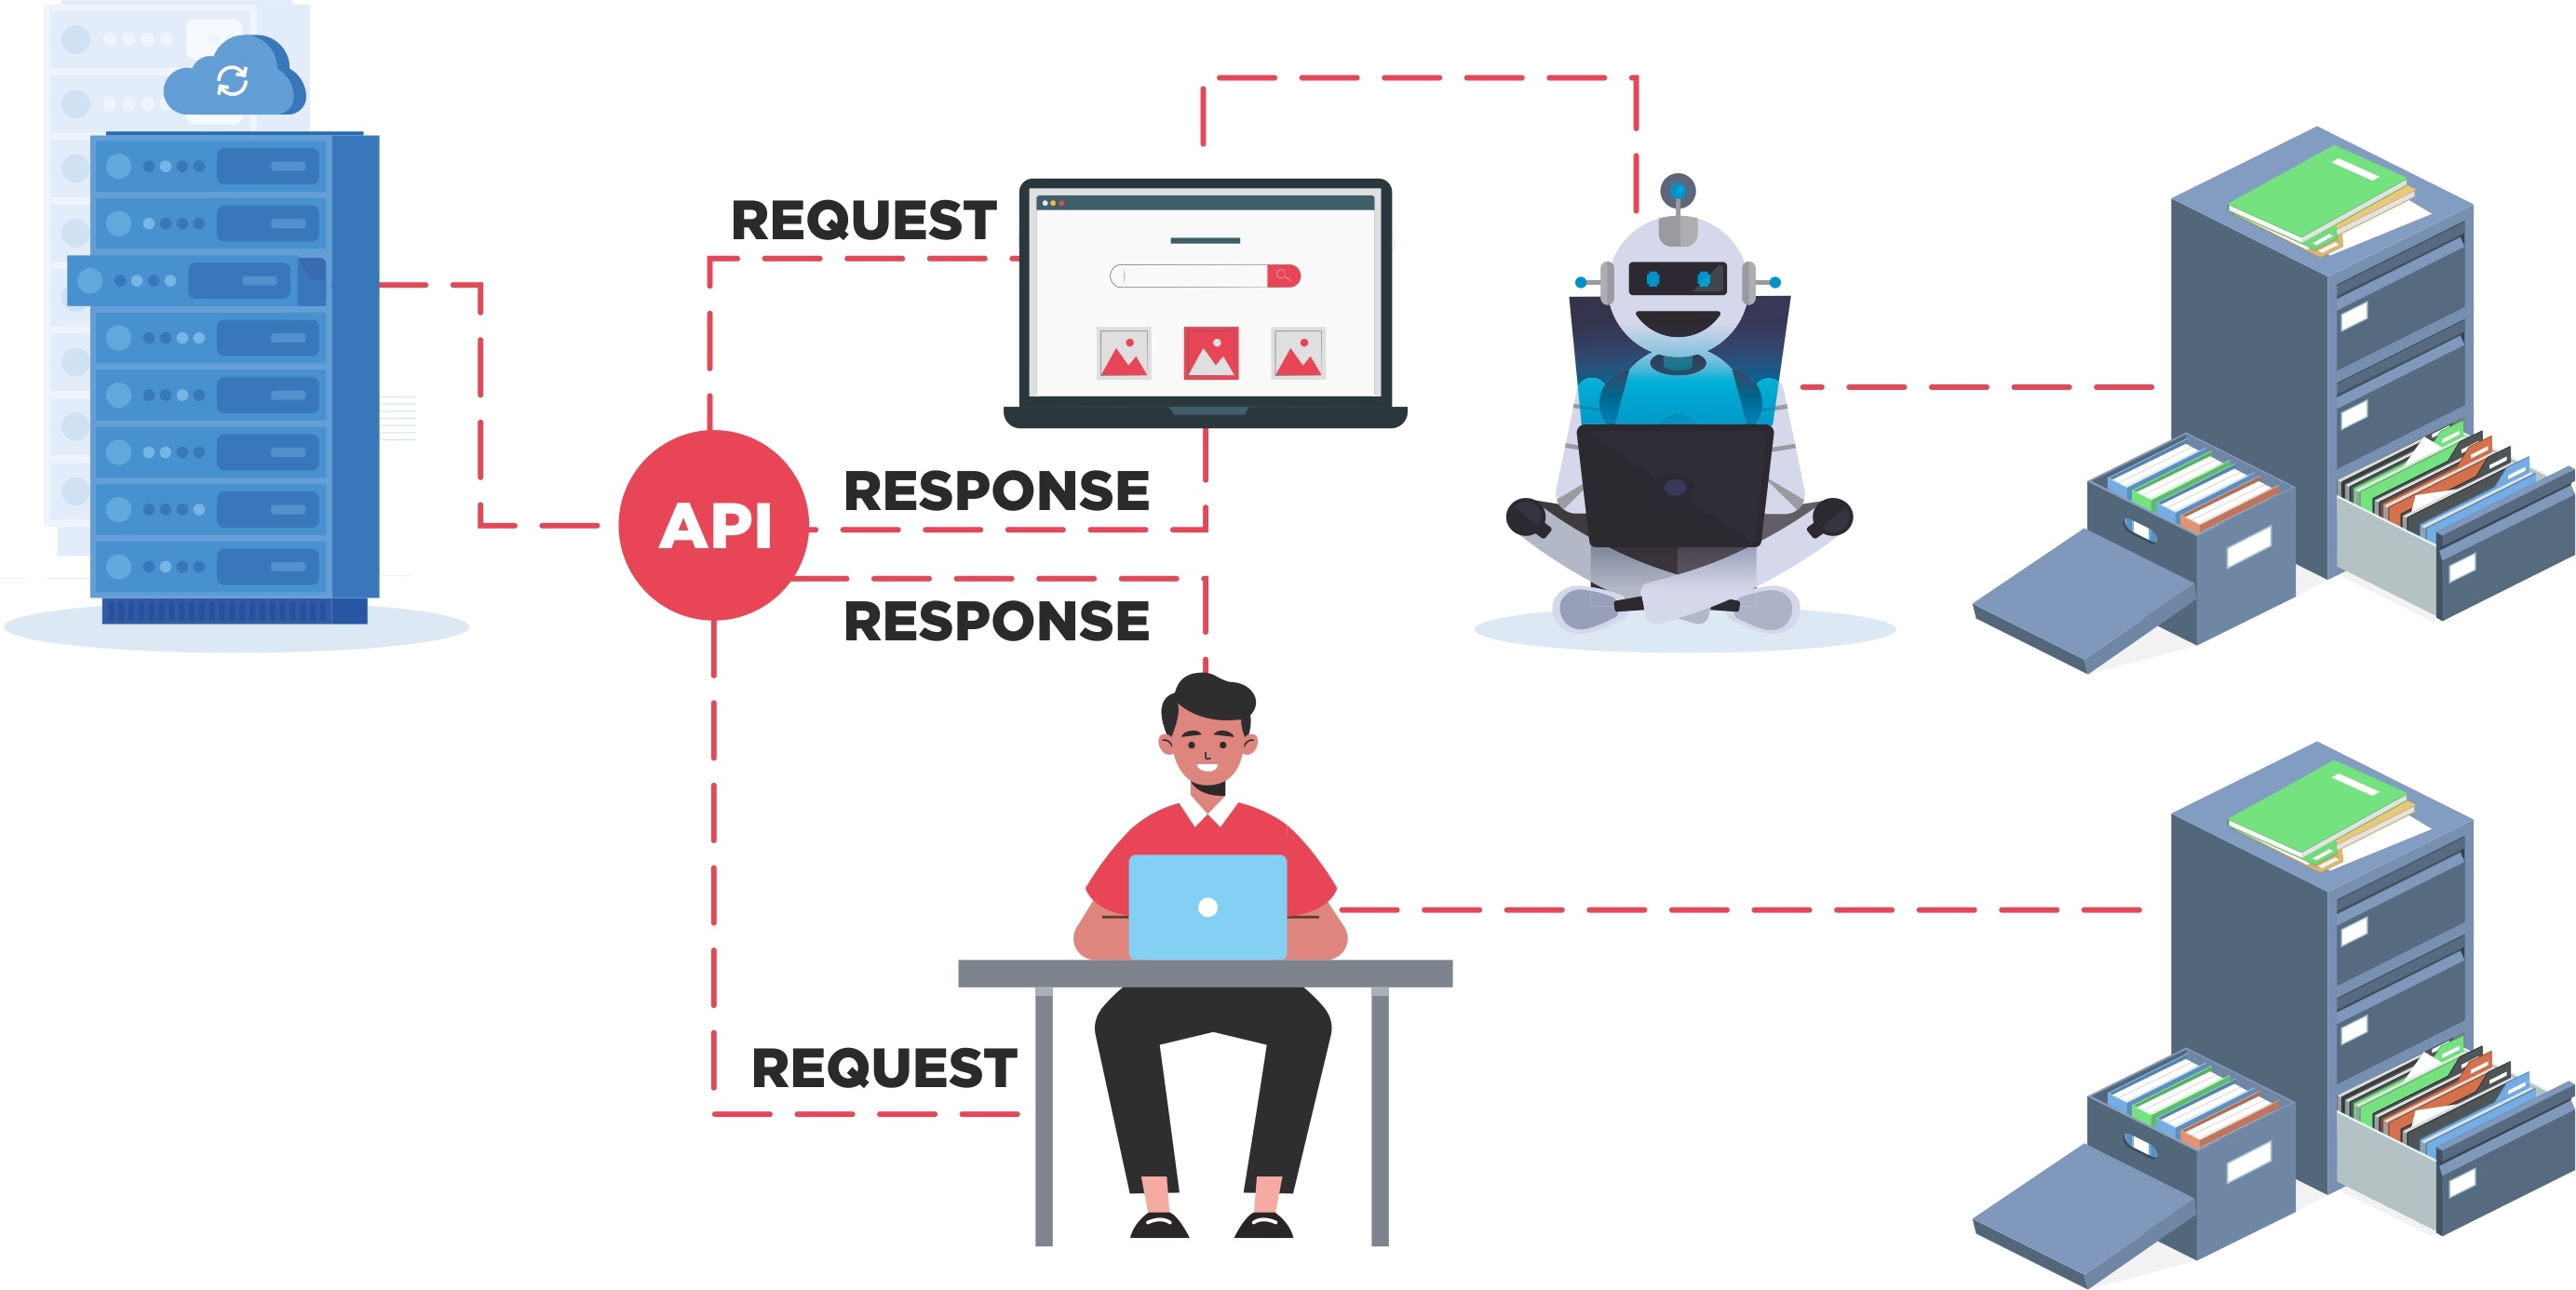
\includegraphics[scale = .4]{png/api.jpg}
        \end{figure}
    }
    \only<+>{
        \begin{figure}
            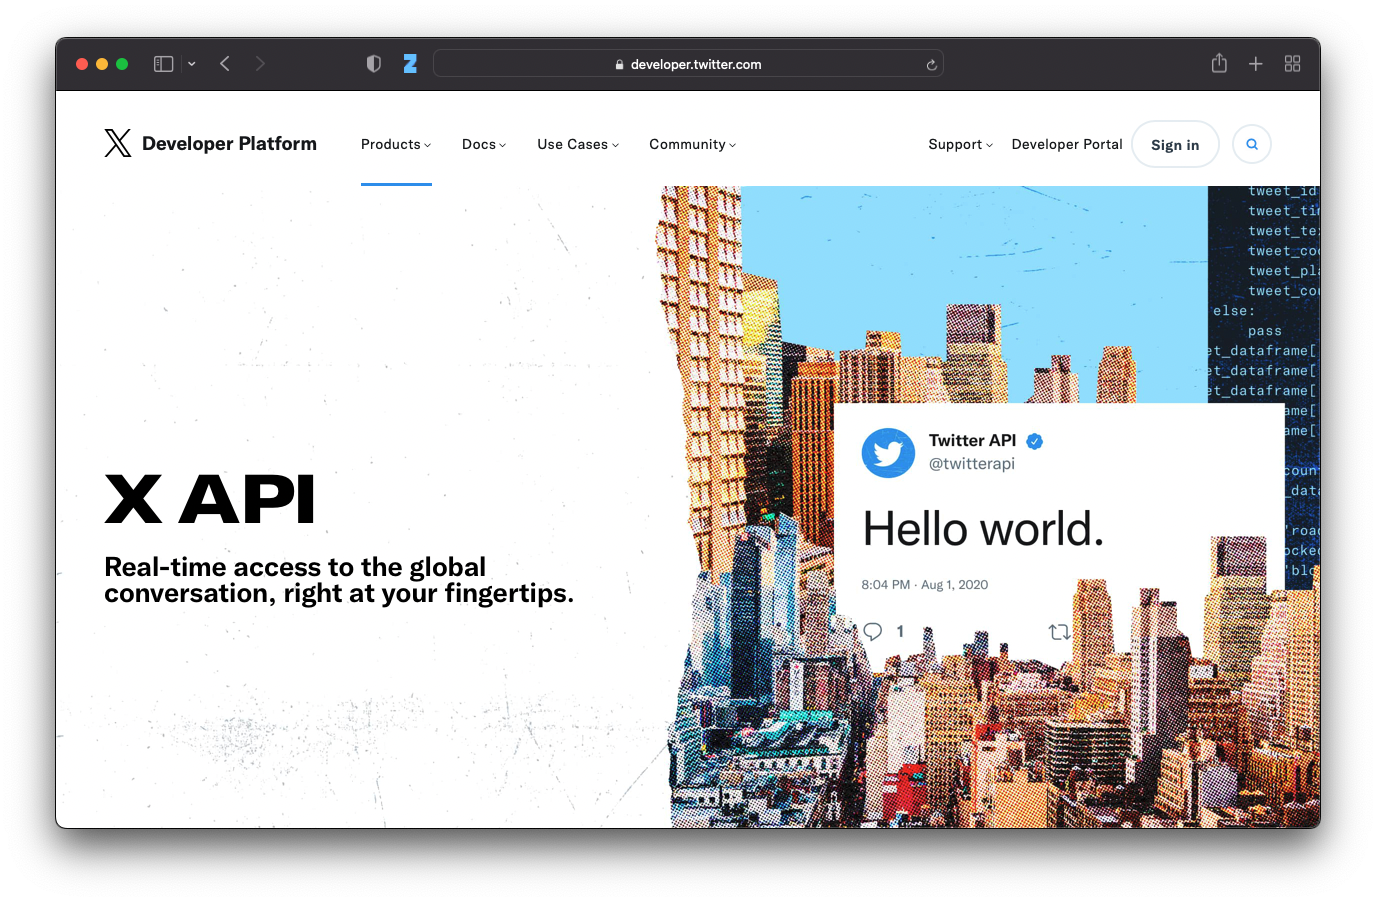
\includegraphics[width = \textwidth]{png/twitter.png}
            \caption{from \textcolor{blue}{\href{https://developer.twitter.com/en/use-cases/analyze}{Developer X}}}
        \end{figure}
    }
    \only<+>{
        \begin{definition}
            \emph{Aplication Programming Interface} is a communication protocol between a client and a server intended to simplify the building of client-side software. In other words, it is a contract between the client and the server which defines the format of possible requests and the format of the response (i.e. format of the data).
        \end{definition}
    }
\end{frame}

\subsection[Data Formats]{Data Formats}

\begin{frame}
    \frametitle{Unstructured and Structured Data}
    \only<+>{
        \begin{figure}
            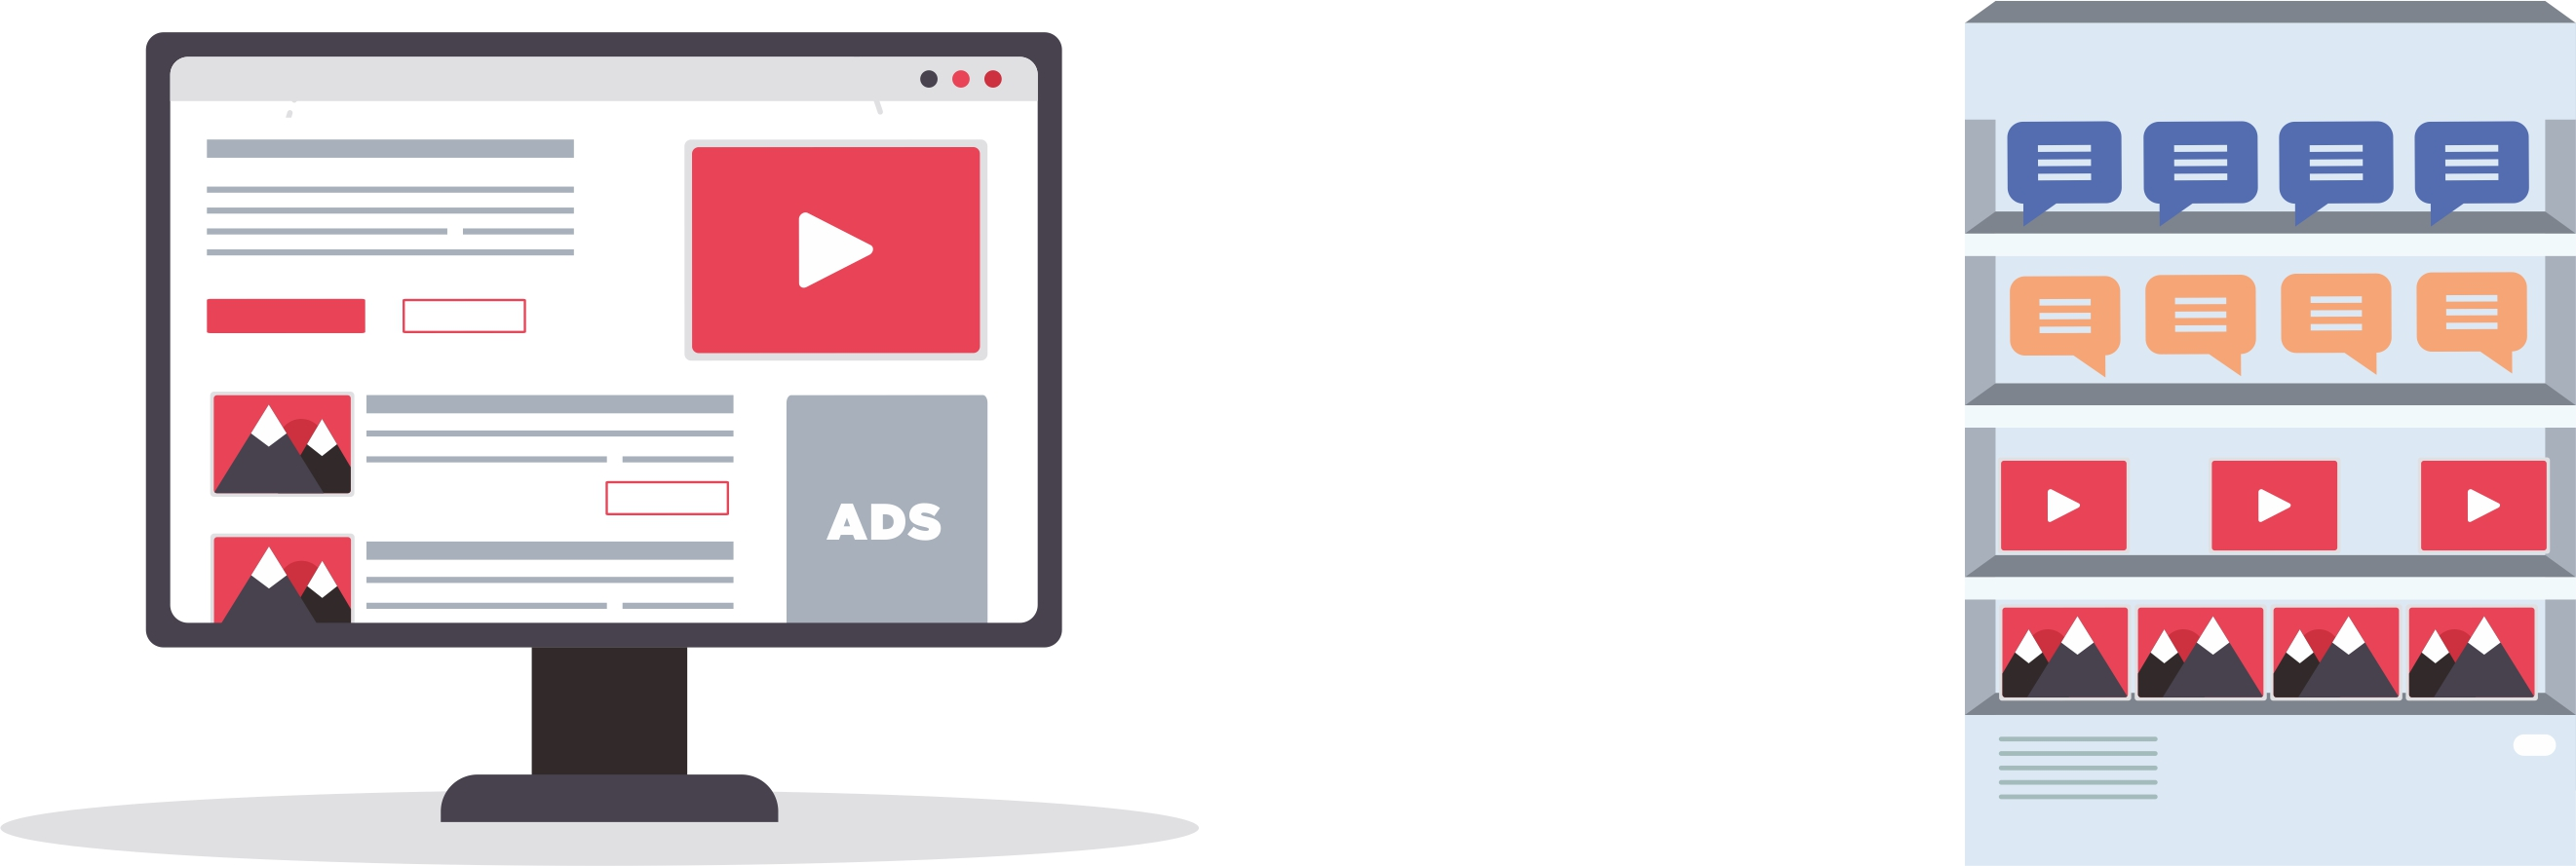
\includegraphics[scale = .4]{png/structured.jpg}
        \end{figure}
    }
    \only<+>{\begin{columns}[t]
        \begin{column}{.5\textwidth}
            Unstructured Data:
            \begin{itemize}
                \item can't be displayed in rows and columns
                \item images, audio, video, e-mails, spreadsheets, etc. (fun staff)
                \item requires more storage
                \item extremely hard to manage and analysis
            \end{itemize}
        \end{column}
        \begin{column}{.5\textwidth}
            Structured Data:
            \begin{itemize}
                \item can be displayed in rows and columns
                \item numbers, text, dates
                \item requires less storage
                \item easy to manage and analysis
            \end{itemize}
        \end{column}
        \end{columns}
    }
    \end{frame}
\begin{frame}
    \frametitle{Data Formats}
    \only<+>{
        Marianna is a 17 years old young lady. Although her main field of interest is physics (especially quantum physics and string theory), she also fancies sports. Her favorite physical activities are fishing and football.
        Marian, on the other hand, is a naughty 15 years old boy who only loves literature, especially Szymborska poems touch his heart.
    }
    \only<+>{
        \textcolor{red}{Marianna} is a \textcolor{blue}{17} years old young lady. Although her main field of interest is \underline{physics} (especially \textbf{quantum physics} and \textbf{string theory}), she also fancies \underline{sport}. Her favorite physical activities are \textbf{fishing} and \textbf{football}.
        \textcolor{red}{Marian}, on the other hand, is a naughty \textcolor{blue}{15} years old boy who only loves \underline{literature}, especially Szymborska \textbf{poems} touches his heart.
    }
    \only<+>{
        \resizebox{\textwidth}{!}{
            \begin{tabular}{l | c | c | c | c | c | c | c | c }
            Name & Sex & Age & Interest A & Interest A1 & Interest A2 & Interest B & Interest B1 & Interest B2\\
            \hline \hline
            Marianna & F & 17 & physics & quantum physics & string theory & sport & fishing & football\\
            Marian & M & 15 & literature & poems & n/a & n/a & n/a & n/a \\
            \end{tabular}}

    }
\end{frame}

\begin{frame}[fragile]{JSON - JavaScript Object Notation}
\begin{minted}[fontsize=\footnotesize]{js}
{
    "name": "Marianna",
    "age": 17,
    "interests": [
        {
            "name": "physics",
            "field": [
                "quantum physics",
                "string theory"
            ]
        },
        {
            "name": "sport",
            "field": [
                "fishing",
                "football"
            ]
        }
    ]
}
\end{minted}
\end{frame}

\begin{frame}[fragile]{JSON - JavaScript Object Notation}
\begin{minted}[fontsize=\footnotesize]{js}
{
    "name": "Marian",
    "age": 15,
    "interests": [
        {
            "name": "literature",
            "genre": [
                "poems"
            ]
        }
    ]
}
\end{minted}
\end{frame}

\begin{frame}
    \frametitle{JSON - JavaScript Object Notation}
    \begin{definition}
        \emph{JavaScript Object Notation} is a lightweight text data format that is relatively easy to read for both the human naked eye and computers. Although it derives from JavaScript it is a language-independent data format. JSON is built on two structures: a collection of key-item pairs and an ordered list of values. JSON filenames use .json extension.
    \end{definition}
\end{frame}


\begin{frame}[fragile]{JSON Lines}
\begin{minted}[fontsize=\footnotesize]{js}
{"name":"Marianna","age":17,"interests":[
    {"name":"physics","field":["quantumphysics","stringtheory"]},
    {"name":"sport","field":["fishing","football"]}
]}
{"name":"Marian","age":15,"interests":[
    {"name":"literature","genre":["poems"]}
]}
\end{minted}
\begin{definition}
    \emph{JSON Lines} (newline-delimited JSON) is a lightweight text data format that can be processed one record at a time. Each line consists of a JSON. JSON Lines filenames use .jl or .jsonl extensions.
\end{definition}
\end{frame}

\section[NLP]{Natural Language Processing}

\begin{frame}
    \frametitle{Natural Language Processing}
    \only<+>{
        \begin{figure}
            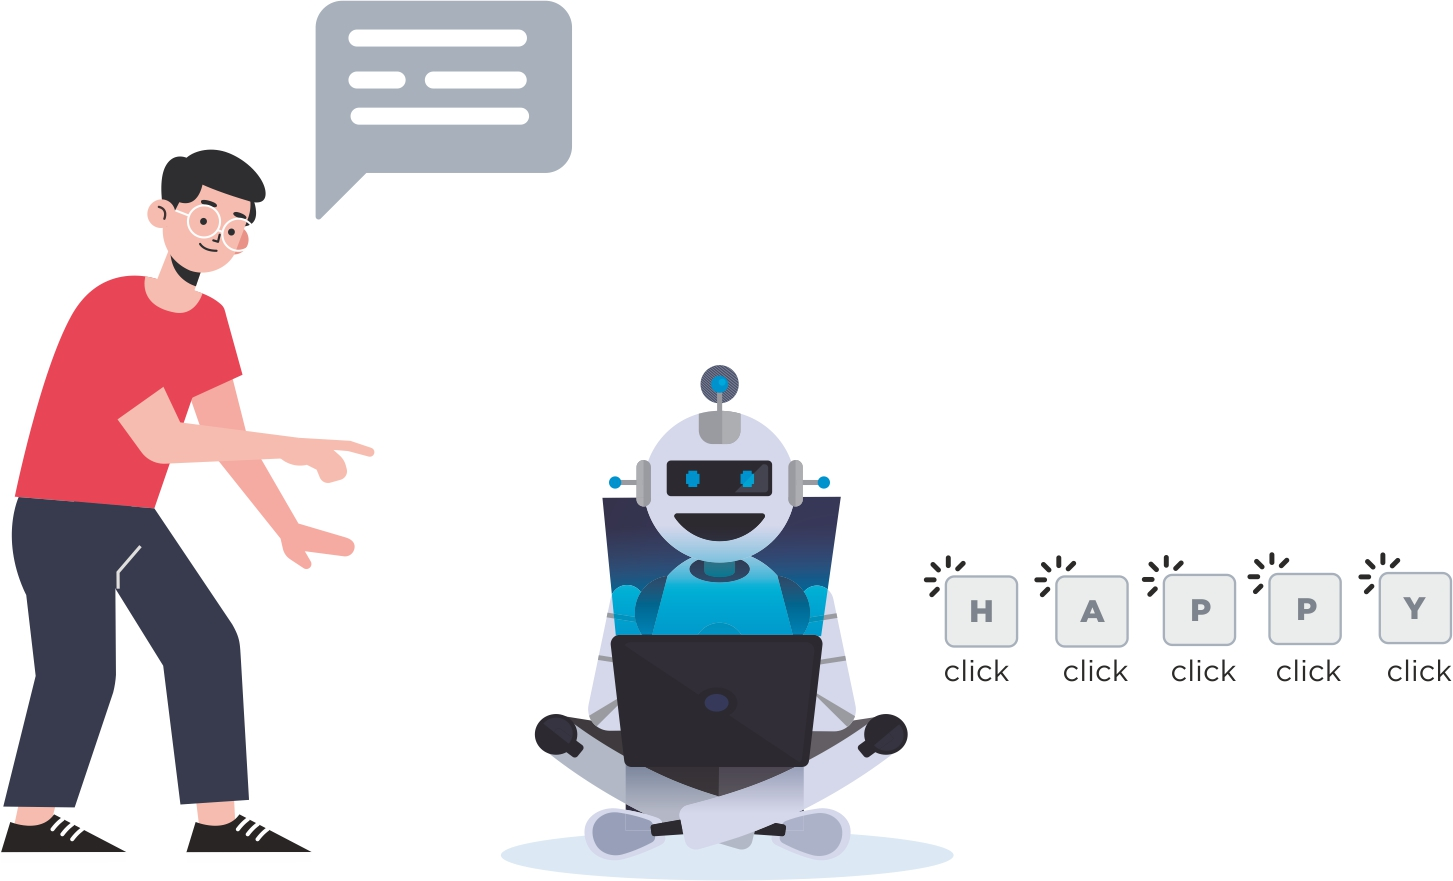
\includegraphics[scale = .7]{png/nlp.jpg}
        \end{figure}
    }
    \only<+>{
        \begin{definition}
            In a general sense \emph{Natural Language Processing} (NLP) is an analytical approach that uses a set of (usually) computer-based methods to extract meaning, topics, or sentiment from natural language data (written or spoken). In other words, it is a set of computer algorithms that tries to synthesize human language.  \end{definition}
    }
    \only<+>{
        \begin{itemize}
            \item tokenization
            \item stemming
            \item lemmatization
            \item sentiment analysis
            \item vector models
            \item topic modeling
            \item part of speech tagging
            \item entities analysis
    \end{itemize}
    }
\end{frame}

\end{document}
